\section{Introduction}


Parking lots present a difficult search problem. Drivers lack the visibility
to determine where spots are available, and may spend a non-trivial amount of
time searching for a spot. The problem is difficult enough that WikiHow
includes directions~\cite{wikihow-park} and the Wall Street Journal has
published an online article~\cite{wsj-park} with tips on spot stalking for
shoppers during the holidays. Searching not only generates frustration but
also wastes energy and produces harmful environmental emissions.

Using technology to address parking availability is not novel.  Key high
demand areas such as downtown parking areas and airport lots frequently sport
instrumentation such as lot access sensors, spot sensors, availability
signage, and payment booths.  Such approaches appear less frequently  in
situations where parking saturation occurs intermittently, if predictably.
In many university campuses, aside from peak class hours, and in suburban
shopping malls, aside from holiday shopping seasons, significant parking
remains unoccupied.  Likely because of this, the installation of a monitoring
infrastructure is presently not justified.

Installation costs for parking systems in existing high demand areas can be
significant:  \$18M for monitoring and collection equipment for 7000 street
spots in the SFPark system.\cite{sf-park}  For lot parking, inexpensive
systems have been proposed that simply track lot counts.\cite{lot-count}  In
practice, a permanant infrastructure for such an approach would involve
permanant mounting and communication for each sensor.  For comparison, the
real cost of an installed vehicle detector including wireless transponder is
about \$9,700.\cite{car-detect}  Communication link costs alone can run
\$4,600.\cite{mstp-park}  Apart from instrumentation, the data collected
needs to be relayed to drivers.  One programmable sign to advertise lot
availability can cost \$50,000.\cite{mstp-park}.  Scaling these figures
compounds the problem:  our own campus setting involves over 40 major lots
with over 80 separate entrances.

***ADD IN CITATIONS...
-new cites:  sf-park, lot-count, car-detect, mstp-park

Online smartphone application stores such as Google Play and the App Store
teem with apps to locate parking spots. Although some drivers may find these
applications useful, the apps either do not provide real-time parking lot
availability or simply display publicly-available information. Several
research projects have attempted to address these limitations~\cite{4212497,
Chen:2012:COS, Delot:2009:CRP, 5062057, Mathur:2010:PDS} but include
requirements rendering them impractical.  They either require additional
infrastructure~\cite{5062057}, on-vehicle equipment~\cite{Mathur:2010:PDS}
or networking~\cite{Delot:2009:CRP, Mathur:2010:PDS}, or onerous manual user
input~\cite{Chen:2012:COS}. In contrast, we believe the solution is already
in peoples' pockets.

We present \textit{PocketParker}, a system that predicts parking lot
availability using smartphones. Unlike previous approaches, PocketParker
requires no additional infrastructure, no vehicle modifications, and no user
input, only installation on a smartphone.  PocketParker runs unattended in
the background and uses the accelerometer to detect parking lot
arrivals and departures.  These are forwarded to a central server, which
incorporates them into per-lot availability models.  This allows PocketParker
to order lots accurately by the probability that they contain an available
spot.  In general, we consider our approach to be an example of a subset of
crowdsourcing that does not require any manual user input, which we call
\textit{pocketsourcing}.

Predicting parking availability requires the efficient and accurate detection
of parking-related events and the incorporation of the effect of
\textit{hidden drivers}---drivers not using PocketParker---into our
availability model. We address the first challenge with a simple yet effective
and energy conserving event detector which uses sense data to record vehicle
arrivals and departures.  The second goal we achieve with an availability
estimator that maintains a probability model for each lot by incorporating
data from PocketParker clients. We use detected events both to estimate
arrival and departure rates.  Even with limited information, there are moments
when PocketParker can be certain about the availability of a parking spot in a
given lot and can use this certainty to assist users find spots.

We perform an evaluation of PocketParker using a variety of methods
tailored to each system component. We evaluate our parking event detector in
a controlled environment with eight volunteers participating in ten parking
scenarios. We design a simulator to evaluate our parking availability
estimator, giving us the flexibility to experiment with a variety of
parameters and parking lot types. We evaluate the overall effectiveness of
PocketParker in a field test involving 105 smartphones users over forty five
days. To obtain ground truth, we deploy four cameras that monitor two parking
lots over two weeks. We inspect and hand-code four days' worth of images of
these lots to measure their true availability. Our results demonstrate the
overall efficiency and accuracy of PocketParker.

PocketParker has several components distributed across users' smartphones and
a backend server. Our paper describes each component in detail. We start by
presenting related work in order to distinguish PocketParker from previous
parking monitoring approaches. The next two sections describe two major
components of PocketParker: our parking event detector and availability model.
The evaluation that follows is based both on simulations, controlled
experiments, and a prototype deployment involving 105 users.  Finally, we
discuss limitations and future work.

\begin{comment}
\begin{figure}
\centering
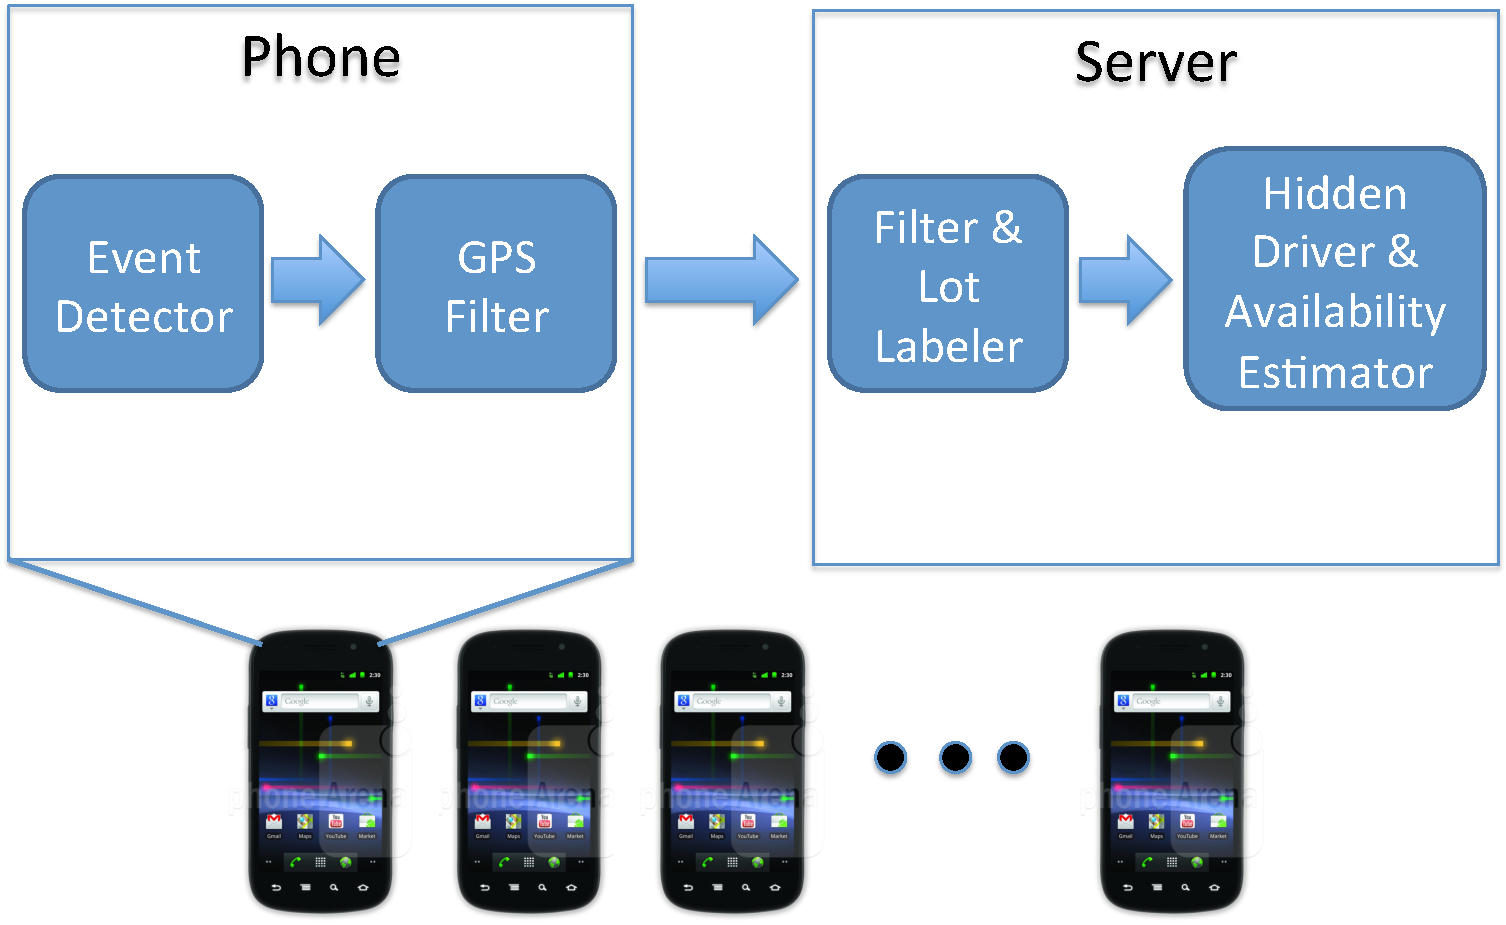
\includegraphics[height=1.5in]{./figures/blockdiagram.pdf}

\caption{\textbf{The PocketParker architecture.} Events generated by an
activity detector running quietly on each smartphone are processed by a
central server and used to estimate parking lot availability.}

\label{fig-arch}
\vspace*{-0.2in}
\end{figure}
\end{comment}
